\documentclass[dvipdfmx,11pt]{beamer}		% for my notebook computer and my Mac computer
%\documentclass[11pt]{beamer}			% for overleaf

\usepackage{amsmath}
\usepackage{amssymb}
%\usepackage{amsthm}
\usepackage{multicol}
\usepackage{listings}
\usepackage{otf}
\usepackage{algorithm}
\usepackage{algorithmic}
\usepackage{tikz}
\usepackage{mathtools}
\usepackage{comment}
\usetheme{Berlin}	%全体のデザイン

\useoutertheme[subsection=false]{smoothbars}	%デザインのカスタマイズ

\setbeamertemplate{navigation symbols}{}	%右下のちっちゃいナビゲーション記号を非表示

\AtBeginSubsection[]	%サブセクションごとに目次を表示
{\begin{frame}{Contents}
    \begin{multicols}{2}
        \tableofcontents[currentsubsection]
    \end{multicols}
\end{frame}}
\newtheorem{defi}{Definition}
\newtheorem{thm}[defi]{Theorem}
\newtheorem{prop}[defi]{Proposition}
\newtheorem{conj}[defi]{Conjecture}
\newtheorem{exam}[defi]{Example}
\newtheorem{prob}[defi]{Problem}
\newtheorem{set}[defi]{Setting}
\newtheorem{claim}[defi]{Claim}

\newcommand{\N}{\mathbb{N}}
\newcommand{\R}{\mathbb{R}}
\newcommand{\X}{\mathcal{X}}
\newcommand{\Y}{\mathcal{Y}}
\newcommand{\Hil}{\mathcal{H}}
\newcommand{\Loss}{\mathcal{L}_{D}}
\newcommand{\MLsp}{(\X, \Y, D, \Hil, \Loss)}

\newcommand{\argmax}{\mathop{\rm arg~max}\limits}
\newcommand{\argmin}{\mathop{\rm arg~min}\limits}


\title{Machine Learning tutorial}
\author{Takaya KOIZUMI}
\institute{Mathematical Science, B4}
\date{Applied Mathematics and Physics informal seminor}
\begin{document}
    \begin{frame}\frametitle{}
        \titlepage
    \end{frame}
    \section*{Contents}
    \begin{frame}\frametitle{Contents}
        \begin{multicols}{2}
            \tableofcontents
        \end{multicols}
    \end{frame}
    \section{機械学習の枠組み}
    \subsection{機械学習とは}
    \begin{frame}\frametitle{機械学習とは}
        機械学習とは, 「関数近似論」である.
        \begin{block}{世の中で機械学習を使って実現したと言われている技術}
            \begin{enumerate}
                \item 翻訳~~($\{$全ての日本語$\}$$\to$$\{$全ての英語$\}$という関数)
                \item メール分類~~($\{$全てのメールの文章$\}$$\to$$\{$迷惑メール, 非迷惑メール$\}$という関数)
                \item 音声認識~~($\{$音声$\}$$\to$$\{$文章$\}$という関数)
            \end{enumerate}
        \end{block}
        もちろん, 間違いを起こすこともある. (大事なメールが, 迷惑メールに入ることも...)
    \end{frame}
    \begin{frame}\frametitle{数学的には}
        前スライドの話を集合論を用いて, もう少し数学的にきちんと書くならば, 以下のようになるだろう.
        \begin{block}{機械学習?}
            $\X$, $\Y$をそれぞれ$\R^d$, $\R^m$の部分集合とする. 
            この時, 良い関数$f:\X\to\Y$を見つけることを機械学習という. 
        \end{block} 
        しかし, この定義には以下の問題がある.
        \begin{block}{上の定義の問題点}
            \begin{enumerate}
                \item 候補となる関数が多すぎる. (ヒントも何もないのに探せない)
                \item 良い関数とは何か, 定義されていない.
            \end{enumerate}
        \end{block}
    \end{frame}
    \subsection{機械学習の数学的定式化へ}
    \begin{frame}\frametitle{前半の問題解消}
        では, まず前半の「候補となる関数が多すぎる.」という問題を解決していこう. \\ \indent
        この問題の解決方法として, 人間がヒント(条件)を与えてあげることで, 関数全ての
        集合ではなく, ある程度絞った集合$\Hil$にするということを考える. この$\Hil$のことを仮設空間(Hyposesis space)と呼ぶ.
        \begin{defi}[仮設空間]
            $\X$, $\Y$をそれぞれ$\R^d$, $\R^m$の部分集合とする. この時, 集合
            \begin{equation*}
                \Hil :=\{f_{w} :\X\to\Y\mid\text{$f_{w}$に関する条件}\}
            \end{equation*}
            のことを仮設空間と呼び, $\X$を特徴量空間, $\Y$をラベル空間と呼ぶ. また, $f_w\in\Hil$を
            仮設と呼ぶ. 
        \end{defi}
    \end{frame}
    \begin{frame}\frametitle{後半の問題解消}
        では, 後半の「良い関数」というものを定義していこう. 
        機械学習において, 良い関数とは, 未知のデータ$X$に対して正しい値$Y$を返す関数である. 
        そのために, 関数$f$に対してその良さを表す指標である汎化誤差を定義する.
        \begin{defi}[汎化誤差, 損失関数]
            $\Hil$を仮設空間, $(\Omega, \mathcal{F}, \mathbb{P})$を確率空間, $\rho$をデータの確率分布とする.
            この時, 汎化誤差$\ell:\Hil\to\R$を, 
            \begin{equation*}
                \ell(f_{\theta}) = \mathbb{E}_{(X, Y)\sim\rho}[l(f_{w}(X), Y)]
            \end{equation*}
            と定義する. ここで, $l:\Y\times\Y\to\R$は損失関数と呼ばれる凸関数である. 
        \end{defi}
    \end{frame}
    \begin{frame}
        \frametitle{損失関数の具体例}
        \begin{block}{損失関数}
            ここで, よく使われる損失関数の例をいくつか述べておく. 
            \begin{enumerate}
                \item 2乗損失関数 $l(y_1, y_2) = (y_1 - y_2)^2$
                \item 交差エントロピー誤差 $l(y_1, y_2) = -y_2\log y_1$
            \end{enumerate}
        \end{block}
        これで, 「良い関数」を作るためには, 汎化誤差$\ell$を最小化させるような仮設空間$\Hil$の元$f$を見つけば良いと言うことになったわけだが, 
        汎化誤差には期待値が含まれるため, 直接最適化させることが難しい. そのため, 持っているデータを利用して別の関数を用意し, その関数を
        最小化することを考える. 
    \end{frame}
    \begin{frame}
        \frametitle{データと経験損失関数}
        \begin{defi}[データ]
            $(\Omega, \mathcal{F}, \mathbb{P})$を確率空間, $\rho$をデータの確率分布とする.
            $\{(X_n, Y_n)\}_{n = 1}^{N}$を$\rho$に従う独立な確率変数列とした時, $\{(X_n, Y_n)\}_{n = 1}^{N}$の観測値$\{(X_n(\omega), Y_n(\omega))\}_{n = 1}^{N}$
            のことをデータ(Data)と呼び, $D = \{(x_n, y_n)\}_{n = 1}^{N}$と表記する.
        \end{defi}
        \begin{defi}[経験損失関数]
            $\Hil$を仮設空間, $D = \{(x_n, y_n)\}_{n = 1}^{N}$をデータ, $l:\Y\times\Y\to\R$を
            損失関数とする. この時, 経験損失関数$\Loss:\Hil\to\R$を,
            \begin{equation*}
                \Loss(f_{w}) = \sum_{n = 1}^{N}l(f_{w}(x_n), y_n)
            \end{equation*}
            と定義する. 
        \end{defi}
    \end{frame}
    \begin{frame}
        \frametitle{機械学習と学習アルゴリズム}
        さて, ここで改めて機械学習を定義しよう.
        \begin{defi}[機械学習, 学習アルゴリズム]
            $\Hil$を仮設空間, $D$をデータ, $\Loss$を経験損失関数とする. この時, 
            アルゴリズム$\mathcal{A}$を用いて, $\Loss$を最小化・最大化させる過程のことを機械学習
            (あるいは単に学習)と呼び, その時のアルゴリズム$\mathcal{A}$のことを学習アルゴリズムと呼ぶ. 
            また, 最適解$f^{*}\in\Hil$を最適仮設と呼び, その時のパラメータ$w^{*}$を最適パラメータと呼ぶ. 
        \end{defi}
        これ以降, 5つ組$(\X, \Y, D, \Hil, \Loss)$をML空間と呼ぶことにする. 
    \end{frame}
    \section{単回帰と重回帰}
    \subsection{単回帰分析}
    \begin{frame}\frametitle{最も基礎的なモデル}
        まず, 最も基礎的な機械学習モデルである単回帰分析を紹介する. 
        \begin{exam}[単回帰分析]
            ML空間$\MLsp$を以下で定義する. $\X = \R$, $\Y = \R$, 
            \begin{align*}
                \Hil &= \{f:\X\to\Y\mid f(x) = wx, w\in\R\},\\
                \Loss(f) &= \sum_{i = 1}^{N}(f(x_i) - y_i)^2.
            \end{align*}
            このML空間$\MLsp$上で,
            \begin{align*}
                \argmin_{f\in\Hil}\Loss(f)
            \end{align*}
            を求める問題を単回帰分析という.
        \end{exam}
    \end{frame}
    \begin{frame}
        \frametitle{SRAの学習}
        SRAは勾配降下法などを用いて解くこともできるが, 今回は解析的に最適パラメータを求める. 
        SRAの経験損失関数は$w$に関して2次関数となっているので, 平方完成を用いると, 
        \begin{equation*}
            f^{*}(x) = w^{*}x, \hspace{20pt} w^* = \frac{\sum_{i = 1}^{N}x_{i}y_{i}}{\sum_{i = 1}^{N}x_{i}^2}
        \end{equation*}
        と定義される$f^*\in\Hil$が最適であることがわかる. 
    \end{frame}
    \subsection{重回帰分析}
    \begin{frame}
        \frametitle{重回帰分析}
        \begin{exam}[重回帰分析]
            ML空間$\MLsp$を以下のように定義する.\\
            $\X = \R^d(N\geq d)$, $\Y = \R$, 
            \begin{align*}
                \Hil &= \{f:\X\to\Y\mid f(x) = W^{\top}x + b, W\in\R^{d}, b\in\R\},\\
                \Loss(f) &= \sum_{i = 1}^{N}(f(x_i) - y_i)^2.
            \end{align*}
            このML空間$\MLsp$上で
            \begin{align*}
                \argmin_{f\in\Hil}\Loss(f)
            \end{align*}
            を求める問題を重回帰分析という.
        \end{exam}
    \end{frame}
    \begin{frame}
        \frametitle{MRAの学習}
        SRAの時と同様に解析的に最適パラメータを求める(簡単のために$b = 0$とする). $X\in\R^{N\times d}$, $\mathbf{y}\in\R^N$を
        $X = [x_1 x_2 \ldots x_N]^{T}$, $\mathbf{y} = (y_{1}, y_{2}, \cdots, y_{N})^{\top}$と定義する. もし$X$が可逆であるとすると, 
        \begin{align*}
            f^{*}(x) = W_*^{\top}x, \hspace{20pt} W_* = (X^\top X)^{-1}X^\top\mathbf{y}
        \end{align*}
        と定義される$f^*\in\Hil$が最適であることがわかる. なお, $b\neq0$の場合も
        デザイン行列$X$を変更し, $w_{0} = b$とすることで, 上記の計算の場合に帰着することができる\cite{PFN}.
    \end{frame}
    \section{過学習と正則化}
    \subsection{多項式回帰}
    \begin{frame}
        \frametitle{基底関数}
        この節では, はじめに多項式回帰を紹介する. 
        その前に基底関数というものを導入する. 
        \begin{defi}[基底関数]
            $\X$を$\R$の部分集合とする. $\X$から$\R$への$C^1$級関数列$\{\phi_{n}\}_{n = 1}^{d}$が
            $\R$上1次独立である時, $\Phi(x) = (\phi_{0}(x), \phi_{1}(x), \ldots, \phi_{d}(x))$で定義される$\Phi:\X\to\R^{d + 1}$
            を基底関数と呼ぶ. 
        \end{defi}
        基底関数を用いることで, 非線形なデータにも対応することができる. 
    \end{frame}
    \begin{frame}\frametitle{多項式回帰}
        \begin{exam}[多項式回帰]
            ML空間$\MLsp$を以下のように定義する.\\
            $\X = \R, \Y = \R$, 
            \footnotesize
            \begin{align*}
                \Hil &= \{f:\X\to\Y\mid f(x) = W^{\top}\Phi(x), W\in\R^{d + 1}\},\\
                \Loss(f) &= \sum_{i = 1}^{N}(f(x_i) - y_i)^2.
            \end{align*}
            \normalsize
            ここで, $\phi_{n}(x) = x^{n}$, $n\in\{0, 1, \cdots, d\}$とする.\\
            このML空間$\MLsp$上で
            \begin{align*}
                \argmin_{f\in\Hil}\Loss(f)
            \end{align*}
            を求める問題を多項式回帰という. 
        \end{exam}
    \end{frame}
    \begin{frame}
        \frametitle{多項式回帰での学習}
            今回も解析的に解くことにする. $X = [\Phi(x_1), \Phi(x_{2}), \cdots, \Phi(x_N)]^{T}\in\R^{N\times d}$とし, 
            $\mathbf{y} = (y_{1}, y_{2}, \cdots, y_{N})^{T}\in\R^{N}$とする. この時, 最適仮説$f^{*}$は
            重回帰分析と同様に$W = (X^\top X)^{-1}X^\top\mathbf{y}$とすれば
            \begin{align*}
                f^{*}(x) = W^{\top}x
            \end{align*}
            である. 
            \begin{block}{学習パラメータとハイパーパラメータ}
                多項式回帰の多項式の次数$d\in\N$や基底関数$\{\phi_{n}\}_{n = 1}^{d}$のように
                コンピュータに学習させるのではなく, 機械学習モデルの設計者が設定するパラメータのことを
                ハイパーパラメータと呼ぶ. 一方, $W\in\R^{d + 1}$のように, データからコンピュータが自動で学習
                するパラメータのことを学習パラメータと呼び, $\Theta$と表す.
            \end{block}
    \end{frame}
    \begin{frame}
        \frametitle{多項式回帰の過学習}
        \begin{columns}[t]
            \begin{column}{0.65\textwidth} 
                \begin{figure}
                    \centering
                    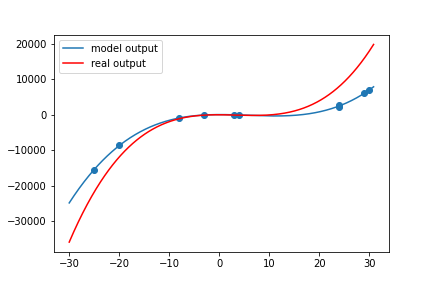
\includegraphics[width = 6.8cm]{Image/overfitting.png}
                    \caption{$d = 3$の時の多項式回帰}
               \end{figure}
            \end{column}
            \begin{column}{0.75\textwidth}
                多項式回帰で学習を行うと左の図\\
                のように, 「教師データには適合し\\ているが, 未知のデータ
                には全く対\\応できない」モデルが学習されて\\しまう. \\
                \indent
                このように, 訓練誤差に対して, \\
                汎化誤差が大きくなってしまう\\
                ことを\textbf{過学習}と呼ぶ. 
            \end{column}
        \end{columns}
    \end{frame}
    \subsection{多項式回帰と正則化}
    \begin{frame}
        \frametitle{正則化}
        過学習を防ぐために, 学習パラメータを制限する方法のことを
        正則化(regularization)と呼ぶ. 具体的には経験損失関数に正則化項と
        いうものを加えて, パラメータが大きくなり過ぎないようにする. 
        \begin{defi}[正則化]
            $\Loss:\Hil\to\R$を経験損失関数とする. $\Loss^{R} := \Loss + L^{R}$とする.
            この時, $\Loss^{R}$を$\Loss$の正則化と呼び, $L^R:\Theta\to\R$を正則化項と呼ぶ.
        \end{defi}
    \end{frame}
    \begin{frame}
        \frametitle{Ridge正則化多項式回帰}
        \begin{exam}[Ridge正則化多項式回帰]
            $\lambda\in\R^{+}\coloneqq\{x\in\R\mid x\geq0\}$, $d\in\N$を任意にとる. 多項式回帰のML空間$\MLsp$の
            経験損失関数を
            \begin{align*}
                \Loss(f) &= \sum_{i = 1}^{N}(f(x_i) - y_i)^2 + \lambda W^\top W
            \end{align*}
            と正則化する. (ここで, $\lambda W^{\top}W$が正則化項である.) 
            このML空間$\MLsp$上で
            \begin{align*}
                \argmin_{f\in\Hil}\Loss(f)
            \end{align*}
            を求める問題をRidge正則化多項式回帰という. 
        \end{exam}
    \end{frame}
    \begin{frame}
        \frametitle{Ridge多項式回帰での学習}
            $X = [\Phi(x_1), \Phi(x_{2}), \cdots, \Phi(x_N)]^{T}\in\R^{N\times d}$とし, 
            $\mathbf{y} = (y_{1}, y_{2}, \cdots, y_{N})^{T}\in\R^{N}$とする. この時, 最適仮説$f^{*}$は
            \begin{align*}
                f^{*}(x) = W_*^{\top}x, \hspace{10pt} W_* = (X^\top X + \lambda I)^{-1}X^\top\mathbf{y}
            \end{align*}
            となる. (ここで, $I$は単位行列である. )
            % あとで計算する.  
    \end{frame}
    \begin{frame}
        \frametitle{正則化の実験}
        \begin{columns}[t]
            \begin{column}{0.65\textwidth} 
                \begin{figure}
                    \centering
                    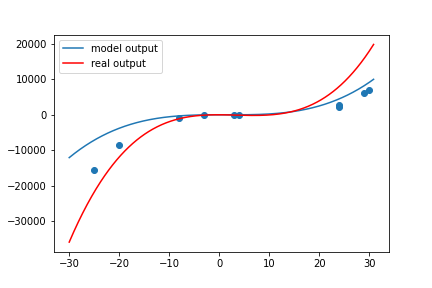
\includegraphics[width = 6.8cm]{Image/regulared.png}
                    \caption{$d = 3$の時のRidge正則化多項式回帰}
               \end{figure}
            \end{column}
            \begin{column}{0.75\textwidth}
                正則化を行うことで, データに完全\\
                にfitせず, 未知のデータにも\\
                ある程度対応できるようになった. \\
                ただ, -10以下のデータに関しては\\
                逆に精度が下がる結果になって\\
                しまった. (方程の方が綺麗...)
            \end{column}
        \end{columns}
    \end{frame}
    \section{ロジスティック回帰}
    \subsection{分類問題とone-hotベクトル}
    \begin{frame}
        \frametitle{分類問題とone-hotベクトル}
        今回は入力データがどのクラスに所属するのかを予測するモデルである「分類」モデルを扱う. 
        そのために, 準備としてソフトマックス関数とone-hotベクトルを導入する. 
        \begin{defi}[ソフトマックス関数]
            $\psi:\R^d\to\R^d$を以下で定義する.
            \begin{align*}
                \psi(x)_{i} = \frac{\exp(x_i)}{\sum_{k = 1}^d\exp(x_k)}
            \end{align*}
            この時, $\psi$をソフトマックス関数と呼ぶ.
        \end{defi}
        \begin{defi}[one-hot ベクトル]
            $y\in\R^m$が第$c\in\{1, 2, \cdots, m\}$成分が1であり, 残りの成分が0である時, 
            $y$をone-hotベクトルという.
        \end{defi}
    \end{frame}
    \begin{frame}
        \frametitle{クラスラベルとone-hotベクトル}
        one-hotベクトルの使い方について解説する. \\
        ジャンケンの手の画像が与えられた時にその手が「グー, チョキ, パー」のうちどれなのかを
        予測するモデルを構築するとする($m = 3$). 
        この時, データセット$\{(x_{n}, y_{n})\}_{n = 1}^{N}\subset \R^{28\times 28}\times\{\text{グー, チョキ, パー}\}$を
        \begin{enumerate}
            \item $y_{i} =$ "グー"なら$y_i = (1, 0, 0)$
            \item $y_{i} =$ "チョキ"なら$y_i = (0, 1, 0)$
            \item $y_{i} =$ "パー"なら$y_i = (0, 0, 1)$
        \end{enumerate}
        として変更し, 新たなデータセット$\{(x_{n}, y_{n})\}_{n = 1}^{N}\subset \R^{28\times 28}\times\R^3$を得る. 
    \end{frame}
    \subsection{ロジスティック回帰と勾配降下法}
    \begin{frame}
        \frametitle{ロジスティック回帰}
        \begin{exam}[$m$値分類ロジスティック回帰]
            ML空間$\MLsp$を以下のように定義する.\\
            $\X=\R^d$, $\Y = \R^m$,
            \footnotesize 
            \begin{align*}
                \Hil &= \{f:\X\to\Y\mid f(x) = \psi(Wx + b), W\in\R^{m\times d}, b\in\R^m\},\\
                \Loss(f) &= -\sum_{n = 1}^{N}\sum_{k = 1}^{m}y_{nk}\log f(x_n)_{k},
            \end{align*}
            \normalsize
            ここで$\psi:\R^m\to\R^m$はソフトマックス関数であり, $y_{n}$はone-hotベクトルである. このML空間$\MLsp$上で
            \begin{align*}
                \argmin_{f\in\Hil}\Loss(f)
            \end{align*}
            を求める問題を$m$値分類ロジスティック回帰という.
        \end{exam}
    \end{frame}
    \begin{frame}
        \frametitle{勾配降下法}
        今回は解析的に, 経験損失関数の解を求めるのではなく, 勾配降下法というアルゴリズムを用いて, 
        解くことにする. 
        \begin{algorithm}[H]
            \caption{Gradient Decent}
            \begin{algorithmic}
                \REQUIRE F: $C^1$ function on $\R^{d}$
                \REQUIRE $0<\alpha<1$ : learning rate 
                \REQUIRE $\theta$: Initial parameter vector
                \STATE $\theta\leftarrow\theta_{0}$
                \WHILE{$\theta$ not converged} 
                \STATE $\theta\leftarrow\theta - \alpha\nabla F(\theta)$ 
                \ENDWHILE
                \RETURN $\theta$
            \end{algorithmic}
        \end{algorithm}
    \end{frame}
    \begin{frame}
        \frametitle{経験損失関数の勾配計算}
        今回の経験損失関数に対して$w_{ij}, b_{i}$についての偏微分を計算すると以下のようになる. 
        \begin{equation*}
            \frac{\partial\Loss}{\partial w_{ij}} = -\sum_{n = 1}^{N}\left(y_{ni} - f(x_{n})_{i}\right)x_{nj}, \hspace{10pt}\frac{\partial\Loss}{\partial b_{i}} = -\sum_{n = 1}^{N}(y_{ni} - f(x_{n})_{i})
        \end{equation*}
        したがって, $X = [x_{1}, x_{2}, \cdots, x_{N}]$, $Y = [y_1, y_2, \cdots, y_N]$, $F = [f(x_1), f(x_2), \cdots, f(x_N)]$, 
        $\mathbf{1} = [1, 1, \cdots, 1]^{\top}\in\R^{N\times 1}$とすれば,
        \begin{equation*}
            \frac{\partial\Loss}{\partial W} = -(Y - F)X^{\top}, \hspace{10pt}  \frac{\partial\Loss}{\partial b} = -(Y - F)\mathbf{1}
        \end{equation*}
        となる. 
    \end{frame}
    \begin{frame}
        \frametitle{クラスラベルの予測方法}
        ロジスティック回帰の最適仮説$f^{*}$が得られた時, $x\in\X$に対してのクラスラベル
        $c\in\{1, 2, \cdots, m\}$を,
        \begin{equation*}
            c = \argmax_{i\in\{1, 2, \cdots, m\}}f(x)_{i}
        \end{equation*}
        として求める. これは, シグモイド関数の出力$\psi(x)$の$i$番目の成分$\psi(x)_i$が
        $x$がクラス$i$に所属する確率であるとみなせることから, 所属する確率が一番高いもの
        を予測値とするのが自然だからである. 
        % https://gensasaki.hatenablog.com/entry/2018/08/30/042807
    \end{frame}
    \subsection{MNISTでの学習結果}
    \begin{frame}
        \frametitle{MNISTでの学習}
        MNISTとは以下のような$28\times28$ピクセルの数字か書かれたデータセットである. 
        \begin{figure}[htbp]
            \begin{minipage}{0.32\hsize}
                \centering
                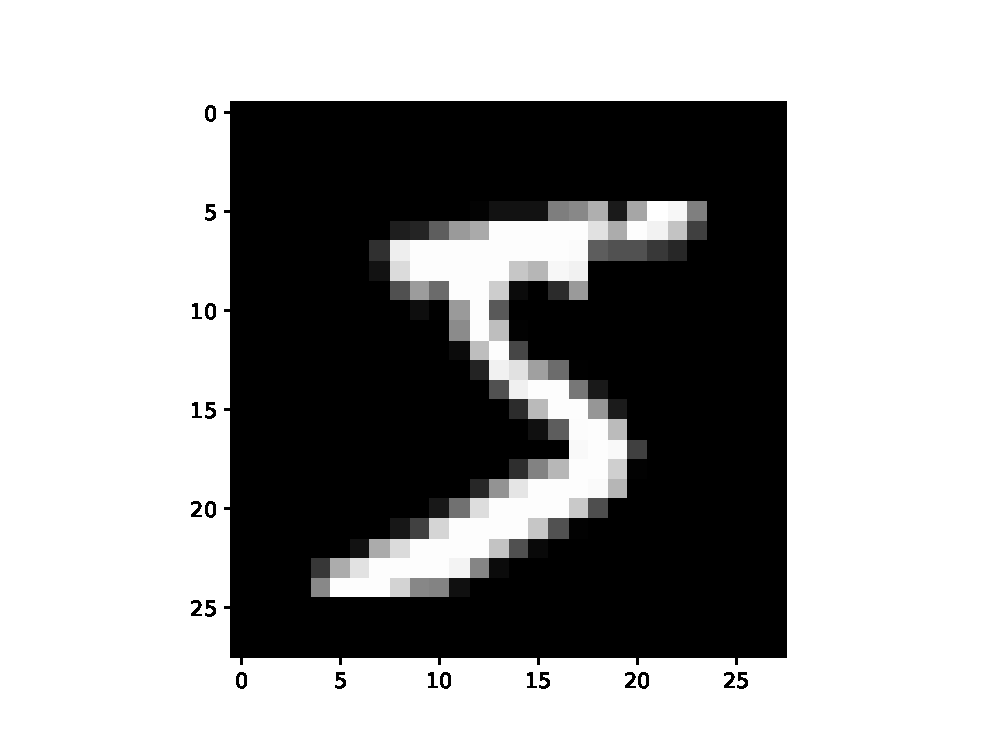
\includegraphics[width = 5.3cm]{Image/MNIST_sample1.eps}
                \caption{数字の5}
            \end{minipage}
            \begin{minipage}{0.32\hsize}
                \centering
                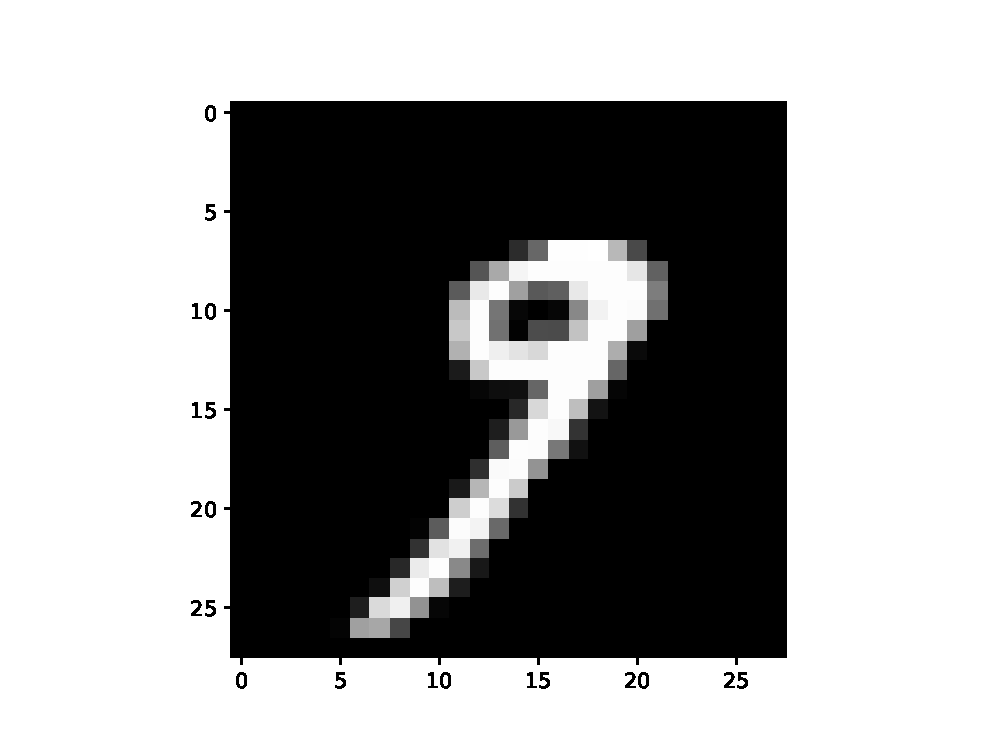
\includegraphics[width = 5.3cm]{Image/MNIST_sample2.eps}
                \caption{数字の9}
            \end{minipage}
            \begin{minipage}{0.32\hsize}
                \centering
                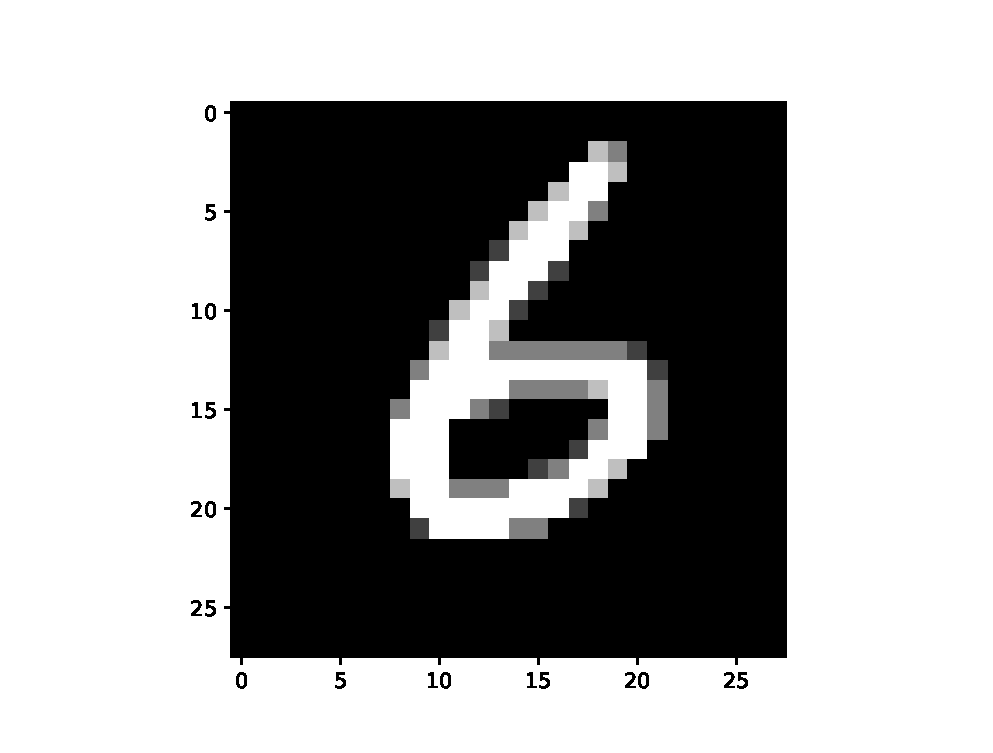
\includegraphics[width = 5.3cm]{Image/MNIST_sample3.eps}
                \caption{数字の6}
            \end{minipage}
        \end{figure}
    \end{frame}
    \begin{frame}
        \frametitle{学習結果}
        \begin{columns}[t]
            \begin{column}{0.65\textwidth} 
                \begin{figure}
                    \centering
                    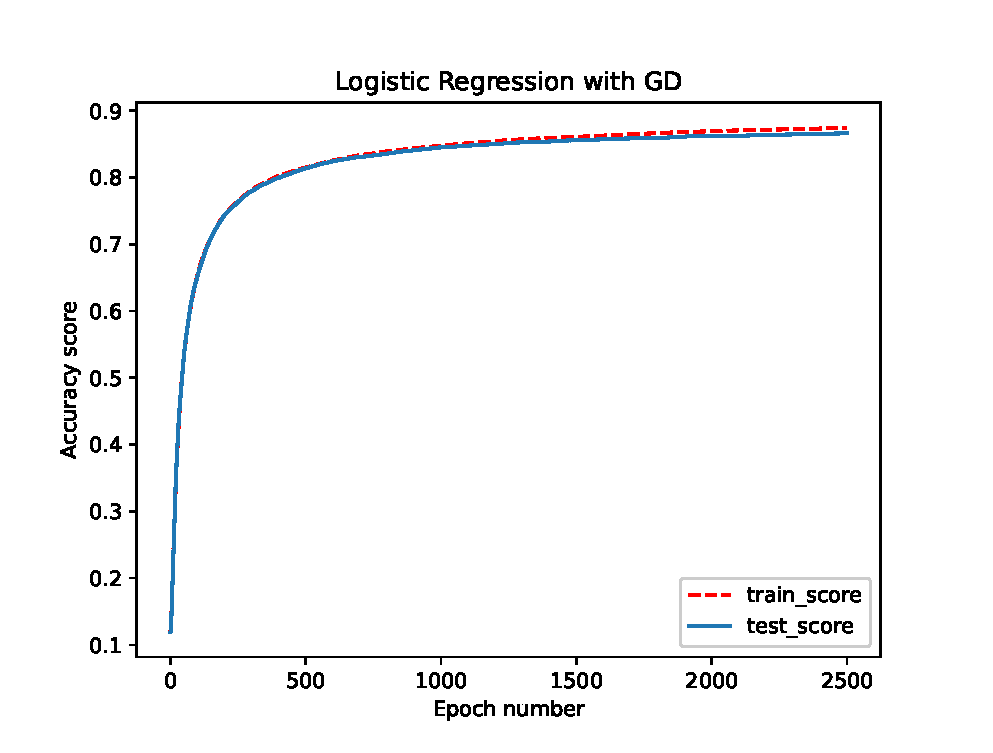
\includegraphics[width = 6.8cm]{Image/MNIST_Experiment.eps}
                    \caption{$\alpha = 0.0001$とした時の, MNSIT実験の結果}
               \end{figure}
            \end{column}
            \begin{column}{0.75\textwidth}
                ロジスティック回帰でMNISTを\\
                学習した結果を左に示す. \\
                テストデータに関しても$85\%$程度\\
                の精度がでた. 
            \end{column}
        \end{columns}
    \end{frame}
    \section{ニューラルネットワークと深層学習}
    \subsection{ニューラルネットワークと活性化関数}
    \begin{frame}
        \frametitle{活性化関数}
        深層学習について紹介する前に活性化関数について紹介する. 
        \begin{defi}[活性化関数]
            $\sigma:\R^{d}\to\R^{d}$を非線形かつ, Lipschitz連続な関数とする. 
            この時, $\sigma$を活性化関数(activation function)という.
        \end{defi}  
        \begin{exam}[活性化関数]
            \begin{align*}
                \sigma(x)_{i} &= \frac{1}{1 + \exp(-x_{i})},\\
                \text{ReLU}(x)_{i} &= \max(x_{i}, 0).
            \end{align*}
            $\sigma$をシグモイド関数(sigmoid function), $\text{ReLU}$を正規化線形関数(Rectified Linear Unit)
            という.
        \end{exam}
    \end{frame}
    \begin{frame}
        \frametitle{回帰型ニューラルネットワーク}
        \begin{defi}[回帰型ニューラルネットワーク]
            ML空間$\MLsp$を以下のように定義する. $L = \{L_{1}, L_{2}, \cdots, L_{K}\}$を自然数列とする.
            $\X = \R^d$, $\Y = \R$, 
            \footnotesize
            \begin{align*}
                \Hil &= \left\{f:\X\to\Y~\middle|
                \begin{array}{l}
                    f(x) = W^{\top}g_{K}\circ\cdots\circ g_{1}(x) + b, g_{i} = \eta(W_{i}x + b_{i})\\
                    W_{i}\in\R^{L_{i}\times L_{i - 1}}, b_{i}\in\R^{L_{i}}, W\in\R^{L_{K}}, b\in\R
                \end{array}
                \right\},\\
                \Loss(f) &= \frac{1}{N}\sum_{i = 1}^{N}(f(x_i) - y_i)^2,
            \end{align*}
            \normalsize
            ここで$\eta$は活性化関数である. $f\in\Hil$を回帰型(全結合)ニューラルネットワーク(Full-connected Neural Network for Regression)
            と呼び, 各$g_{i}$を$f$の第$i$層(layer)と呼ぶ.
        \end{defi}
    \end{frame}
    \begin{frame}
        \frametitle{分類型ニューラルネットワーク}
        \begin{defi}[分類型ニューラルネットワーク]
            ML空間$\MLsp$を以下のように定義する. $L = \{L_{1}, L_{2}, \cdots, L_{K}\}$を自然数列とする.
            $\X = \R^d$, $\Y = \R^{m}$, 
            \footnotesize
            \begin{align*}
                \Hil &= \left\{f:\X\to\Y~\middle|
                \begin{array}{l}
                    f(x) = \psi(W g_{K}\circ\cdots\circ g_{1}(x) + b), g_{i} = \eta(W_{i}x + b_{i})\\
                        W_{i}\in\R^{L_{i}\times L_{i - 1}}, b_{i}\in\R^{L_{i}}, W\in\R^{m\times L_{K}}, b\in\R^{m}
                \end{array}
                \right\},\\
                \Loss(f) &= -\sum_{n = 1}^{N}\sum_{k = 1}^{m}y_{nk}\log f(x_n)_{k},
            \end{align*}
            \normalsize
            ここで$\eta$は活性化関数, $y_{i}$はone-hotベクトル, $\psi$はソフトマックス関数である. $f\in\Hil$を分類型(全結合)ニューラルネットワーク(Full-connected Neural Network for Classification)
            と呼び, 回帰型の時と同様に各$g_{i}$を$f$の第$i$層と呼ぶ.
        \end{defi}
    \end{frame}
    \begin{frame}
        \frametitle{深層学習}
        以下, ニューラルネットと書けば, 分類, 回帰ニューラルネットワークのいずれかを表すものとする. 
        \begin{defi}[Deep Learning]
            ニューラルネットワークが$K \geq 3$の時に
            \begin{align*}
                \argmin_{f\in\Hil}\Loss(f)
            \end{align*}
            を求める問題を深層学習(Deep Learning)と呼ぶ.
        \end{defi}
    \end{frame}
    \subsection{ニューラルネットワークと普遍性定理}
    \begin{frame}
        \frametitle{Universal Approximation Theorem}
        ニューラルネットの近似能力に関する定理としては, 以下のような定理が知られている. 
        \begin{thm}[普遍性定理\cite{UAT}]
            $\X=[0, 1]^{n}$, $\Hil$を$K = 1$の時の回帰型ニューラルネットの仮説空間とする. 
            この時, 活性化関数$\eta$がシグモイド的関数ならば, 
            \begin{align*}
                \forall f\in C(\X), \forall\varepsilon> 0, \exists G\in\Hil\text{ s.t. } \sup_{x\in\X}|f(x) - G(x)| < \varepsilon
            \end{align*}
            が成立する. 
        \end{thm}
        証明にはHahn・Banachの定理とLieszの表現定理を用いる. 
    \end{frame}
    \begin{frame}
        \frametitle{理論 vs. 実験}
        ニューラルネットワークについてはまだまだわかっていないことが多く, 理論と実験結果が合わないような
        こともしばしばある. 具体的には, 以下のようなものがある.
            \begin{enumerate}
                \item 学習がうまくいく(深層学習の目的関数は非凸関数(局所最適解やプラトーが多く存在する))
                \item 層を増やしたほうが精度が向上する(一般に, モデルを複雑にしすぎると過学習を引き起こす)
            \end{enumerate}
    \end{frame}
    \section*{References}
    \begin{frame}\frametitle{References}
        \begin{thebibliography}{9}
            \beamertemplatetextbibitems
            \bibitem{UAT} G. Cybenko, Approximation by Superpositions of a Sigmoidal Function, 
                            Mathmatics of control, signal and systems, vol. 2, no. 4, 1989
		    \bibitem{PFN} Preferred Networks, ディープラーニング入門 Chainer チュートリアル,
            https://tutorials.chainer.org/ja/index.html, 2019
	    \end{thebibliography}
    \end{frame}
\end{document}


